\documentclass[a4paper,12pt]{ctexart}

% Page layout
\usepackage{geometry}
\geometry{a4paper,left=2cm,right=2cm,top=2cm,bottom=2cm,headheight=14.5pt}

% XeLaTeX fonts
\usepackage{fontspec}
\usepackage{xeCJK}
\setCJKfamilyfont{kai}{KaiTi}[AutoFakeBold=true]
\newcommand{\kai}{\CJKfamily{kai}}
\setCJKmainfont{SimSun}[AutoFakeBold=true]
\setCJKsansfont{SimHei}[AutoFakeBold=true]
\setCJKmonofont{FangSong}
\setmainfont{Times New Roman}[
  BoldFont = Times New Roman Bold,
  ItalicFont = Times New Roman Italic,
  BoldItalicFont = Times New Roman Bold Italic
]

% Mathematics
\usepackage{amsmath,amssymb}
\usepackage{unicode-math}
\setmathfont{TeX Gyre Termes Math}
\newcommand{\bm}[1]{\symbf{#1}}
\newcommand{\matr}[1]{\mathbf{#1}}

% Figures and tables
\usepackage{graphicx}
\graphicspath{{figures/}}
\usepackage{float}
\usepackage{caption}
\usepackage{subcaption}
\usepackage{array}
\usepackage{booktabs}
\usepackage{multirow}
\usepackage{tabularx}

% Lists and code
\usepackage{enumitem}
\newlist{mynum}{enumerate}{1}
\setlist[mynum]{label=\arabic*), leftmargin=*}
\usepackage{verbatim}
\usepackage{xcolor}
\usepackage{listings}
\lstset{
  language=C++,
  basicstyle=\ttfamily\small\fontsize{10}{8}\selectfont\bfseries,
  keywordstyle=\color{blue},
  commentstyle=\color{green!60!black}\fontspec{SimSun}\addfontfeature{LetterSpace=-1},
  morecomment=[l]{//},
  morecomment=[s]{/*}{*/},
  stringstyle=\color{red},
  numbers=left,
  numberstyle=\tiny\color{gray},
  stepnumber=1,
  numbersep=5pt,
  backgroundcolor=\color{white},
  showspaces=false,
  showstringspaces=false,
  showtabs=false,
  frame=single,
  tabsize=4,
  captionpos=b,
  breaklines=true,
  breakatwhitespace=true,
  escapeinside={\%*}{*)},
  morekeywords={NaN, isnan, stod, cerr, cout, endl, cin, ifstream, ofstream, istringstream},
  texcl=true,
  columns=fixed,
  basewidth=0.5em
}

% Spacing and paragraphs
\usepackage{setspace}
\setstretch{1.35}
\setlength{\parindent}{2em}
\setlength{\parskip}{0pt}

% Section headings
\ctexset{
  section = {
    name={,、},
    number=\chinese{section},
    format={\zihao{3}\bfseries\heiti},
    aftername=,
  },
  subsection = {
    format={\zihao{4}\bfseries\heiti},
  },
  subsubsection = {
    format={\zihao{-4}\bfseries\heiti}
  }
}

% Header and footer
\usepackage{fancyhdr}
\fancypagestyle{plain}{%
  \fancyhf{}
  \fancyhead[L]{\small 室内定位技术·结课报告}
  \renewcommand{\headrulewidth}{0.4pt}
  \fancyfoot[C]{\thepage}
}
\pagestyle{plain}

% Table of contents
\usepackage[titles]{tocloft}
\renewcommand{\cftdot}{.}
\renewcommand{\cftdotsep}{0.5}
\renewcommand{\cftsecleader}{\cftdotfill{\cftdotsep}}

% Hyperlinks
\usepackage[unicode]{hyperref}
\hypersetup{
  colorlinks=true,
  linkcolor=black,
  citecolor=black,
  urlcolor=blue,
  pdfborder={0 0 0},
  pdfstartview=FitH
}

% Cover support
\usepackage{tikz}
\usepackage{attachfile2}


\begin{document}
    \thispagestyle{empty}

% ---------- 武汉大学图片 ----------
\begin{center}
	\vspace*{2cm}  % 上方间距
	
\includegraphics[width=7cm]{figures/WHU大字.JPG}  %插入图片，宽度5cm（可调整）
	\vspace{2cm}   % 图片下方间距
\end{center}

% ---------- 标题：结课实验报告 ----------
\begin{center}
	{\fontsize{24pt}{30pt}\selectfont \textbf{\kai 室内定位技术结课报告}} \\[3cm]   % 大字号，换行后间距1cm
\end{center}

% ---------- 实验报告名称 ----------
\begin{center}
	{\Large \textbf{《室内定位技术》}} \\[3cm]  % 加粗，换行后间距1.5cm
	
\end{center}

% ---------- 学生信息 ----------
\begin{center}
	
	\begin{tabular}{@{\hspace{4em}}l}
		学生姓名：尚之琦 \\ [0.5cm]
		学生学号：2024302142059 \\ [0.5cm]
		指导老师：李由 \\ [0.5cm]
		专业名称：导航工程（智能导航实验班） \\[0.5cm]
		课程名称：室内定位技术
	\end{tabular}
\end{center}



% ---------- 日期 ----------
\vfill
\begin{center}
	{\fontfamily{ptm}\selectfont 二〇二六年十一月} \\
\end{center}

% ---------- 分页符（可选，若需后续内容分页） ----------
\newpage
\mbox{}  % 空页面（仅分页符时可用）



    \pagenumbering{Roman}

%     \begin{abstract}
% 本文基于室内定位课程实验代码与配套数据，分析并评价三类定位方法：基于超声测距的几何交会、基于 Wi-Fi 接收信号强度（RSS）的指纹匹配，以及基于手机惯性与磁场传感器的行人航迹推算（PDR）。几何定位采用已知基站坐标下的非线性最小二乘迭代；指纹方法由参考点 RSS 均值构成数据库，并通过共同可见接入点的加权 K 近邻估计位置；PDR 程序从姿态调平、磁航向/陀螺航向计算到步伐检测和固定步长轨迹积分。对可隔离复算的指纹算法，本报告在原始训练与测试数据上重新计算，50 个历元均输出位置，水平误差均值为 1.128 m、RMSE 为 1.422 m。教室超声数据依据给定的 C++ 结果文件与参考轨迹按时间对齐复核，7,086 个历元的平面位置 RMSE 为 0.239 m。PDR 数据采用项目中已有 C++ 运行结果作后处理核验，按照参考经纬度的局部切平面坐标与步伐时刻对齐，误差 RMSE 为 8.381 m；这一数值反映本次轨迹、参考坐标和方向/初始对准共同作用的差异，不应解释为仅由传感器噪声造成的纯算法误差。报告同时讨论各输出的证据来源、可比性边界和实现局限。
%     \end{abstract}
%     \noindent\textbf{关键词：} 室内定位；距离交会；RSS 指纹；航迹推算；误差评价

    \tableofcontents
    \clearpage

    \pagenumbering{arabic}

    \section{研究背景与实验目标}
卫星导航在室内环境中会受到遮挡、反射与衰减影响，难以持续提供稳定的米级定位。课程内容从定位传感器、几何定位、航迹推算、数据库匹配扩展到运动约束、多源融合和机器学习。本实验选择项目中已有数据和程序覆盖的三条技术路线，重点考察它们的观测量、误差传播与适用条件，而不是把所有课件主题都误当作已完成的实验。

实验目标是：（1）从代码和数据字段还原真实算法，而非仅按目录名称推断；（2）对具有独立输入的数据复现计算，或对现有程序输出进行可追溯复核；（3）以参考位置评价定位误差，并区分测距残差、轨迹末点偏差等不同指标；（4）指出实验的可重复性、坐标对准和参数标定限制。

\section{环境、数据与证据范围}
项目代码使用 C++17 实现距离交会和 PDR，Python 实现 RSS 指纹及传感器绘图/转换。计算与绘图脚本运行于 Python 3 环境，依赖 NumPy、Matplotlib；C++ 工程 README 指定支持 C++17 的编译器。当前报告的独立复算脚本位于 \texttt{analysis.py}，所有本报告新增图表和统计文件保存在本目录，原始数据与代码未修改。

\begin{table}[htbp]
\centering
\caption{数据与本报告分析用途}
\label{tab:data}
\begin{tabular}{p{3.0cm}p{5.3cm}p{5.2cm}}
\toprule
数据集 & 结构与观测 & 本报告中的用途及限制 \\
\midrule
距离交会：教室超声 & 基站坐标、逐历元测距、逐历元参考位置（CSV/文本） & 复核项目已有 C++ 位置输出；参考位置按时间线性插值，评价二维误差。输出文件是项目既有结果，本次未在原目录重新运行 C++。 \\
RSS 指纹 & 97 个参考点坐标、1,989 条建库 RSS 记录、50 条带参考坐标测试记录；每条包含 30 个 AP 通道，缺失值为 $-110$ dBm & 按现有 Python 算法在独立脚本中重新建库、定位和统计误差。 \\
PDR & 6,829 行、约 0.05 s 间隔的 12 列传感器矩阵；588 个带时间戳的参考经纬度位置 & 对项目 C++ 已保存的定位轨迹进行独立对齐和误差统计；不声称本轮重新编译运行 PDR C++。 \\
Android 采集样例 & 采集 App 的传感器、Wi-Fi 和 GPS/KML 记录，包含陀螺、加速度、磁场、Wi-Fi 扫描等 & 用于说明采集链和数据转换用途。该样例不等同于本报告指纹库/PDR 数据，未把它混入定位精度统计。 \\
无人机、UWB、学生超声数据 & 多组基站和测距文件，部分带高度、真值或遮挡分组 & 代码包含对应处理程序；本报告不报告这些组的精度，因为本次没有在隔离副本中运行其 C++ 主程序并完成真值口径核验。 \\
\bottomrule
\end{tabular}
\end{table}

指纹训练文件按参考点编号和 30 个 RSS 数值组织，测试文件另含时间与三维参考坐标。PDR 的传感器矩阵列顺序由读取实现确认：时间、三轴角速度、三轴加速度、三轴磁场以及两个未参与定位的字段。代码将角速度从度每秒转为弧度每秒，将磁场数值乘 $10^{-7}$ 转为特斯拉。距离交会教室程序读取四个基站以及各历元测距/参考数据；输出字段中的 \texttt{range\_rms\_m} 表示测距拟合残差。

    \section{理论模型与程序实现}
\subsection{距离交会与非线性最小二乘}
设第 $i$ 个基站坐标为 $\bm{s}_i=(x_i,y_i,z_i)^T$，待求位置为 $\bm{p}$，观测距离满足
\begin{equation}
 d_i=\|\bm{p}-\bm{s}_i\|+\epsilon_i .
 \label{eq:range}
\end{equation}
当目标高度已知时，可将未知量约化为平面坐标 $(x,y)$；教室程序直接采用二维模型。对当前估计 $\bm{p}_k$，令预测距离 $r_i=\|\bm{p}_k-\bm{s}_i\|$、残差 $l_i=d_i-r_i$，距离函数的雅可比行为 $\bm{h}_i^T=(\bm{p}_k-\bm{s}_i)^T/r_i$。线性化后通过正规方程求改正量
\begin{equation}
 (\bm{H}^T\bm{H})\Delta\bm{p}=\bm{H}^T\bm{l},\qquad
 \bm{p}_{k+1}=\bm{p}_k+\Delta\bm{p}.
 \label{eq:gn}
\end{equation}
代码以参与计算的基站中心作为初值，最多迭代 50 次，位置改正小于 $10^{-4}$ m 时停止，并以法方程行列式/高斯消元枢轴判断退化。无人机程序先将局部范围内的经纬度投影到以首个基站为原点的局部平面，再在已知高度下解二维问题；UWB 程序使用八个基站和三维未知量。此类最小二乘对异常测距敏感，当前实现没有鲁棒核或按观测方差加权。

\subsection{RSS 指纹匹配}
参考点 $j$ 的 AP $a$ 有效观测均值为
\begin{equation}
 \bar r_{j,a}=\frac{1}{n_{j,a}}\sum_{q\in\mathcal{V}_{j,a}} r_{q,a},
 \label{eq:rss-mean}
\end{equation}
其中缺失值 $-110$ 不参与平均。对测试向量 $\bm{r}$，仅在双方共同有效的 AP 集合 $\mathcal{C}_j$ 上计算 RSS 均方根差 $D_j$，并定义覆盖率 $c_j=|\mathcal{C}_j|/|\mathcal{V}|$。代码使用相似度 $w_j=c_j/(1+D_j)$，选择最高分的 $K=3$ 个候选並按得分加权坐标：
\begin{equation}
 \hat{\bm{p}}=\frac{\sum_{j\in\mathcal{N}_K} w_j\bm{p}_j}
 {\sum_{j\in\mathcal{N}_K}w_j}.
 \label{eq:knn}
\end{equation}
此分数是匹配启发式，不是概率；共同 AP 少于 3 时不参与候选。均值指纹压缩了同一位置的时变分布，且算法未对不同 AP 的方差标准化，因此环境变化与强弱 AP 的尺度差异可能影响邻居次序。

\subsection{PDR 航向、步检与位置递推}
程序先由加速度计算横滚、俯仰角，对姿态角做 1 s 滑动平均，再使用课件对应的旋转变换将陀螺和磁场向量调平。航向来源包括调平后的磁强计方位和陀螺竖直分量积分；后者具有零偏累积。步伐检测使用加速度模的波谷阈值 $9.2\,\mathrm{m/s^2}$ 和最小步间隔 $0.30$ s。每检测到一步，程序以固定步长 $L=0.70$ m 更新水平位置：
\begin{equation}
 E_k=E_{k-1}+L\sin\psi_k,\qquad
 N_k=N_{k-1}+L\cos\psi_k,
 \label{eq:pdr}
\end{equation}
其中 $\psi_k$ 为步伐时刻航向。代码还尝试对 $z$ 轴角速度加 $0.25^\circ/\mathrm{s}$ 的试验补偿。源码注释明确该值未经过标定，故只能视作参数敏感性试验，不能称为已估计的零偏。

\section{实验设计与结果}
为核对实验图表覆盖度，先将实例报告图 1--15 与本报告内容逐张对应。图 1 为课程技术路线总览，属于课程组织示意；图 2 为开发环境截图，不是数据结果；图 3--5 分别示意距离交会、PDR 与 KNN 原理；图 6--7 展示 UWB 标签估计/真值的三维及平面轨迹，图 8--11 展示 PDR 惯性观测、姿态角、磁/陀螺航向和步伐检测，图 12--13 对比 PDR 航向补偿前后的轨迹；图 14--15 展示指纹定位轨迹及不同 K 的比较。表~\ref{tab:figure-map} 记录了本报告的重绘证据与未重绘原因。实例图只用于梳理展示逻辑，图形和数值均由本项目数据重新生成。

\begin{table}[htbp]
\centering\small
\caption{实例报告图表与本报告图表对照清单}\label{tab:figure-map}
\begin{tabular}{p{1.0cm}p{4.2cm}p{4.7cm}p{3.0cm}}
\toprule
实例图 & 图示内容及作用 & 本报告对应图表 & 重绘状态/数据依据 \\
\midrule
1 & 课程技术路线，说明内容组织 & 本报告理论与实验章节结构 & 不作为实验图重绘 \\
2 & IDE 运行截图，展示开发环境 & 无 & 界面截图与实验结果无关，不复用 \\
3 & 距离交会几何示意，解释测距定位 & 式~\ref{eq:range}--\ref{eq:gn}及教室轨迹 & 公式说明替代示意图 \\
4 & PDR 原理流程/步进示意 & 式~\ref{eq:pdr}、图~\ref{fig:pdr-signals} & 以真实传感器与步检结果展示 \\
5 & KNN 原理示意，说明邻居加权 & 式~\ref{eq:knn}、图~\ref{fig:k-sensitivity} & 公式与真实 K 对照替代示意 \\
6 & UWB 标签估计与真值三维轨迹 & 图~\ref{fig:uwb}平面轨迹；图~\ref{fig:uwb-z}垂向分量 & 以平面轨迹和独立高度/误差图展示三维偏差 \\
7 & UWB 平面轨迹及 RMSE/DOP 随时间 & 图~\ref{fig:uwb}、图~\ref{fig:uwb}误差子图 & 轨迹和误差重绘；没有可核验 DOP 序列，未绘制 DOP \\
8 & PDR 加速度、角速度、磁场时序 & 图~\ref{fig:pdr-raw}与图~\ref{fig:pdr-signals} & 三轴原始传感器与处理后步伐/航向并列展示 \\
9 & PDR 横滚、俯仰角随时间 & 图~\ref{fig:pdr-signals} & 重绘平滑横滚/俯仰，单位为度 \\
10 & 磁航向与陀螺积分航向 & 图~\ref{fig:pdr-signals}、图~\ref{fig:pdr} & 重绘项目已有输出中的航向序列 \\
11 & 步伐检测位置/时刻 & 图~\ref{fig:pdr-signals} & 以标记叠加在加速度模曲线上 \\
12 & PDR 校正前轨迹与参考路径 & 图~\ref{fig:pdr}、图~\ref{fig:pdr-error} & 重绘磁航向与补偿陀螺轨迹 \\
13 & PDR 校正后轨迹与参考路径 & 图~\ref{fig:pdr}、图~\ref{fig:pdr-error} & 重绘并补充步时刻误差曲线 \\
14 & RSS 指纹定位轨迹 & 图~\ref{fig:fingerprint} & 使用原始训练/测试记录重算 \\
15 & 不同 K 的指纹误差对比 & 图~\ref{fig:k-sensitivity} & 尝试 K=1,2,3,5,7,10 的同一测试集对照 \\
\bottomrule
\end{tabular}
\end{table}

    \subsection{教室超声测距结果复核}
教室数据由四个固定基站的平面坐标、逐时刻测距及参考轨迹组成。程序对每个历元迭代求解位置。本报告读取项目已有的 \texttt{result\_classroom\_cpp.csv}，按时间戳将 \texttt{ref\_pos.txt} 的参考坐标线性插值到解算时刻，然后计算平面误差 $e_k=\|\hat{\bm p}_k-\bm p_k^{\rm ref}\|$。所以本节是对随项目提供的 C++ 输出做后处理复核，不是本轮对 C++ 程序重新编译执行的声称。

\begin{figure}[htbp]
\centering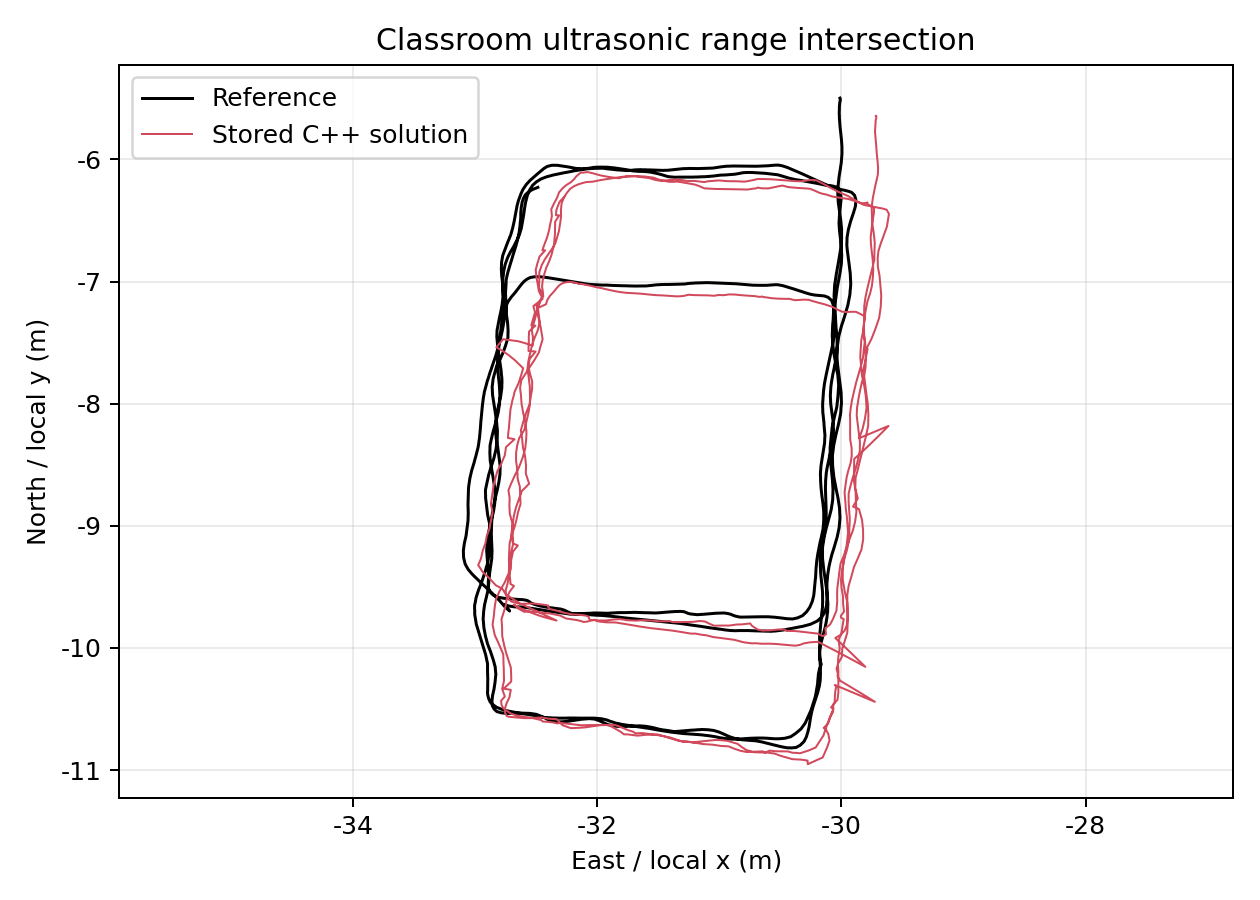
\includegraphics[width=.78\linewidth]{classroom_range_track.png}
\caption{教室超声定位轨迹及时间插值参考轨迹}
\label{fig:classroom}
\end{figure}
图~\ref{fig:classroom-error} 将按时间匹配的水平位置误差与测距拟合 RMS 并列展示。横轴为相对时间，左图纵轴为相对参考轨迹的二维坐标误差，右图纵轴为测距方程残差。两者不是同一误差量：本次位置 RMSE 为 0.239 m，而测距残差中位数仅 0.0099 m；残差较小不保证位置必然准确，因为基站几何构型和参考位置插值误差不会由残差直接反映。误差峰值 0.658 m 应结合时间同步、测距多径和参考采样间隔进一步核查。
\begin{figure}[htbp]
\centering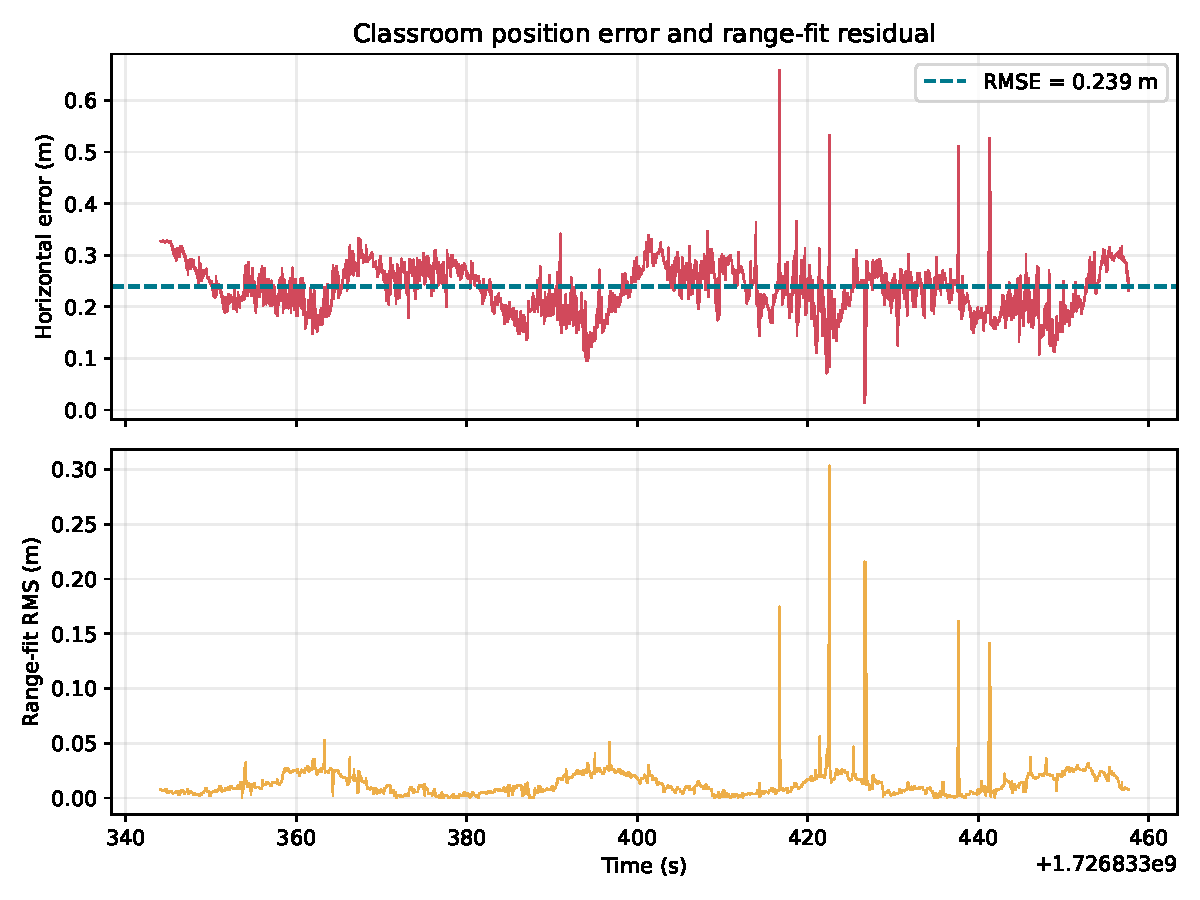
\includegraphics[width=.88\linewidth]{classroom_error_residual.pdf}
\caption{教室超声水平位置误差与测距拟合残差时序}
\label{fig:classroom-error}
\end{figure}
有效解共 7,086 个，按每历元平面误差计算的均值为 0.234 m，RMSE 为 0.239 m，95 分位为 0.304 m，最大值为 0.658 m。测距拟合残差 RMS 的中位数为 0.0099 m。后一个量表示距离方程拟合程度，不能替代位置误差；当基站几何构型不利时，小测距残差仍可能对应较大的位置不确定度。最大位置误差也可能受真值采样插值、基站坐标误差、超声多径/遮挡及时间同步影响。

\subsection{RSS 指纹定位复算}
独立脚本读取 97 个参考点和 1,989 条建库记录，逐 AP 忽略缺失值求均值，再逐个处理 50 个带真值测试时刻。定位函数不接收参考坐标；真值仅在输出位置确定后参与评价。全部 50 个时刻至少存在三个共同有效 AP，故成功率为 100\%。结果轨迹见图~\ref{fig:fingerprint}，误差累计分布见图~\ref{fig:cdf}。

\begin{figure}[htbp]
\centering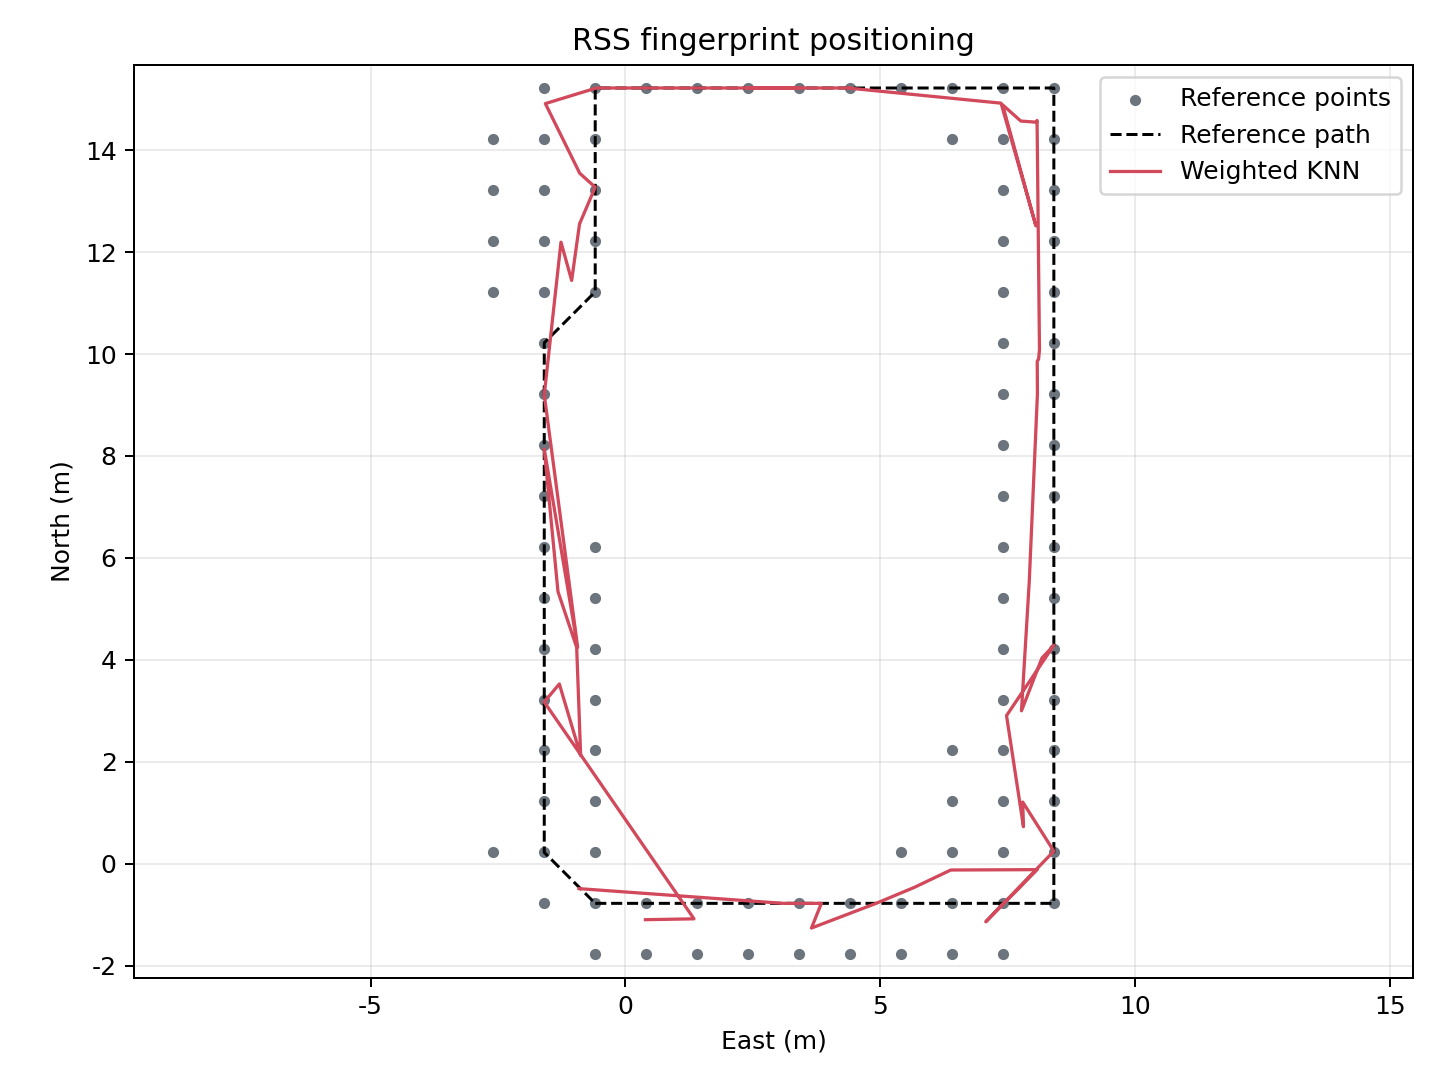
\includegraphics[width=.78\linewidth]{fingerprint_track.png}
\caption{RSS 加权 K 近邻结果与参考轨迹}
\label{fig:fingerprint}
\end{figure}
\begin{figure}[htbp]
\centering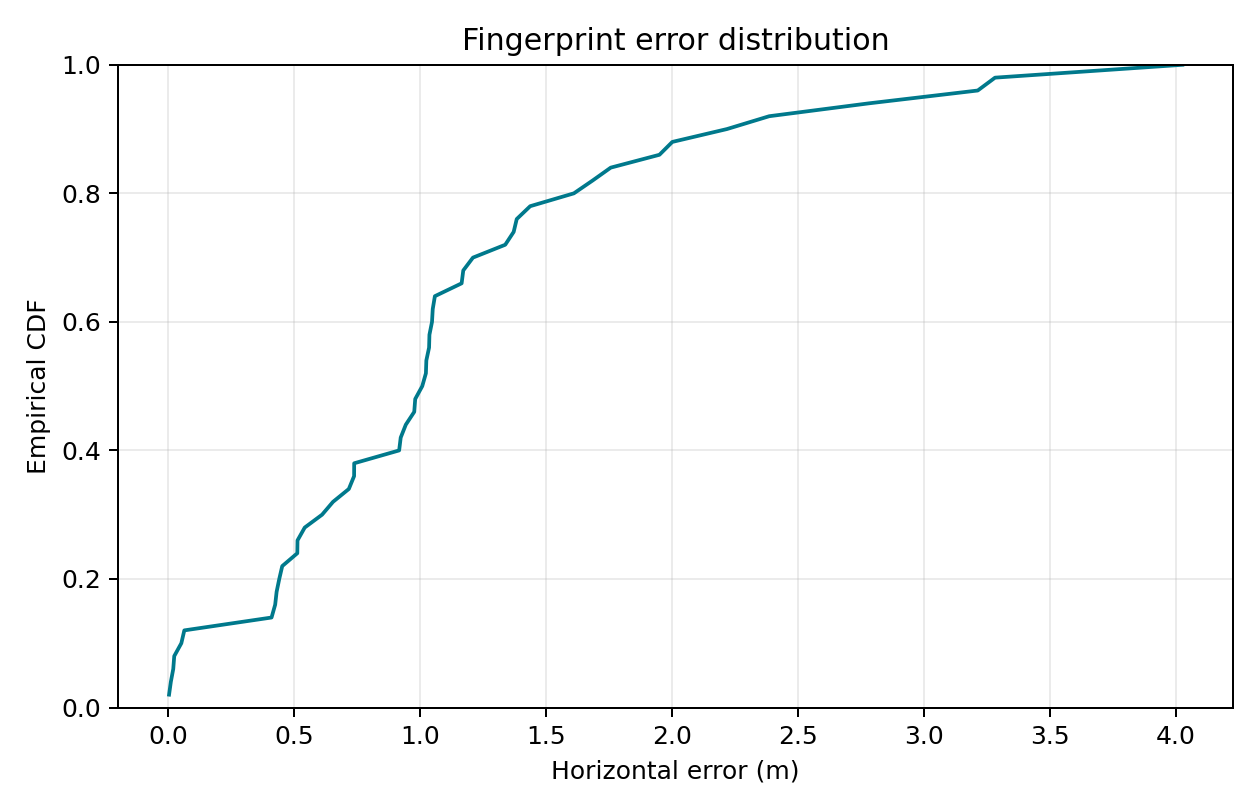
\includegraphics[width=.68\linewidth]{fingerprint_cdf.png}
\caption{指纹水平误差经验累计分布}
\label{fig:cdf}
\end{figure}
\begin{table}[htbp]
\centering\caption{RSS 指纹测试集水平误差统计}\label{tab:finger}
\begin{tabular}{lr}\toprule 指标 & 数值（m）\\\midrule
平均误差 & 1.128\\水平 RMSE & 1.422\\中位数 & 1.016\\95 分位 & 3.020\\最大值 & 4.027\\\bottomrule\end{tabular}
\end{table}
平均误差和 RMSE 的差异显示少数较大误差对平方损失有明显贡献；最大误差约 4 m，说明平均指纹匹配会在 RSS 相似但空间相距较远的位置发生混淆。参考点并非规则完整网格（共 97 点），其空间覆盖不均也使加权坐标插值受采样几何约束。测试路径包含转向段，局部 RSS 的可辨识性和测试采集方向/人体遮挡均可能变化。当前单次测试集规模只有 50 历元，不能据此推断跨设备、跨日期或跨建筑的泛化性能。
为量化邻居数对定位的影响，图~\ref{fig:k-sensitivity} 在完全相同的训练库、距离分数和 50 个测试历元上改变 $K$，误差统计列于表~\ref{tab:k-sensitivity}。$K=1$ 时 RMSE 为 1.311 m，$K=3$ 时为 1.422 m，$K=10$ 时增至 1.725 m；在此小测试集和当前加权规则下，纳入更多邻居会把 RSS 相近但空间位置不同的参考点带入平均，产生位置平滑偏移。该结论只描述本测试集，不能推导出普遍最优的 $K$。
\begin{figure}[htbp]
\centering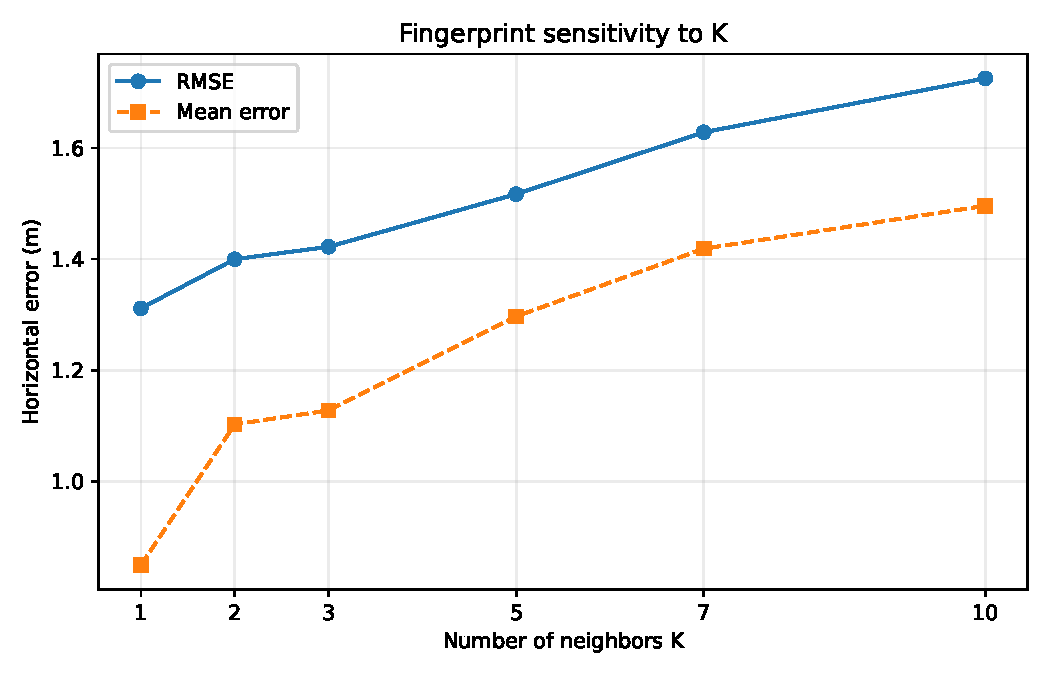
\includegraphics[width=.72\linewidth]{fingerprint_k_sensitivity.pdf}
\caption{指纹加权 KNN 对邻居数 $K$ 的敏感性}
\label{fig:k-sensitivity}
\end{figure}
\begin{table}[htbp]
\centering\caption{不同邻居数下的指纹定位误差}\label{tab:k-sensitivity}
\begin{tabular}{rrrrr}\toprule $K$ & 样本数 & 平均误差（m） & RMSE（m） & 95\%分位（m）\\\midrule
1 & 50 & 0.849 & 1.311 & 3.000\\
2 & 50 & 1.103 & 1.400 & 2.900\\
3 & 50 & 1.128 & 1.422 & 3.020\\
5 & 50 & 1.297 & 1.517 & 2.689\\
7 & 50 & 1.419 & 1.628 & 2.913\\
10 & 50 & 1.496 & 1.725 & 3.280\\\bottomrule\end{tabular}
\end{table}

\subsection{PDR 轨迹与参考位置对照}
本报告没有在原始目录重跑 C++ PDR 主程序，因为它固定写入源码树内的输出目录。为保持原工程只读，采用项目现存的 \texttt{pdr\_result.csv}（6,829 个历元）作为程序输出，对其作独立后处理；参考轨迹由 588 个时间标记的经纬度样本按首点构造局部切平面坐标，并线性插值到步伐时刻。共有 592 个检测步伐，时间覆盖 0 至 341.4 s。该比较包含起始坐标系对准、航向零方向、固定步长模型和参考轨迹插值等共同影响。

\begin{figure}[htbp]
\centering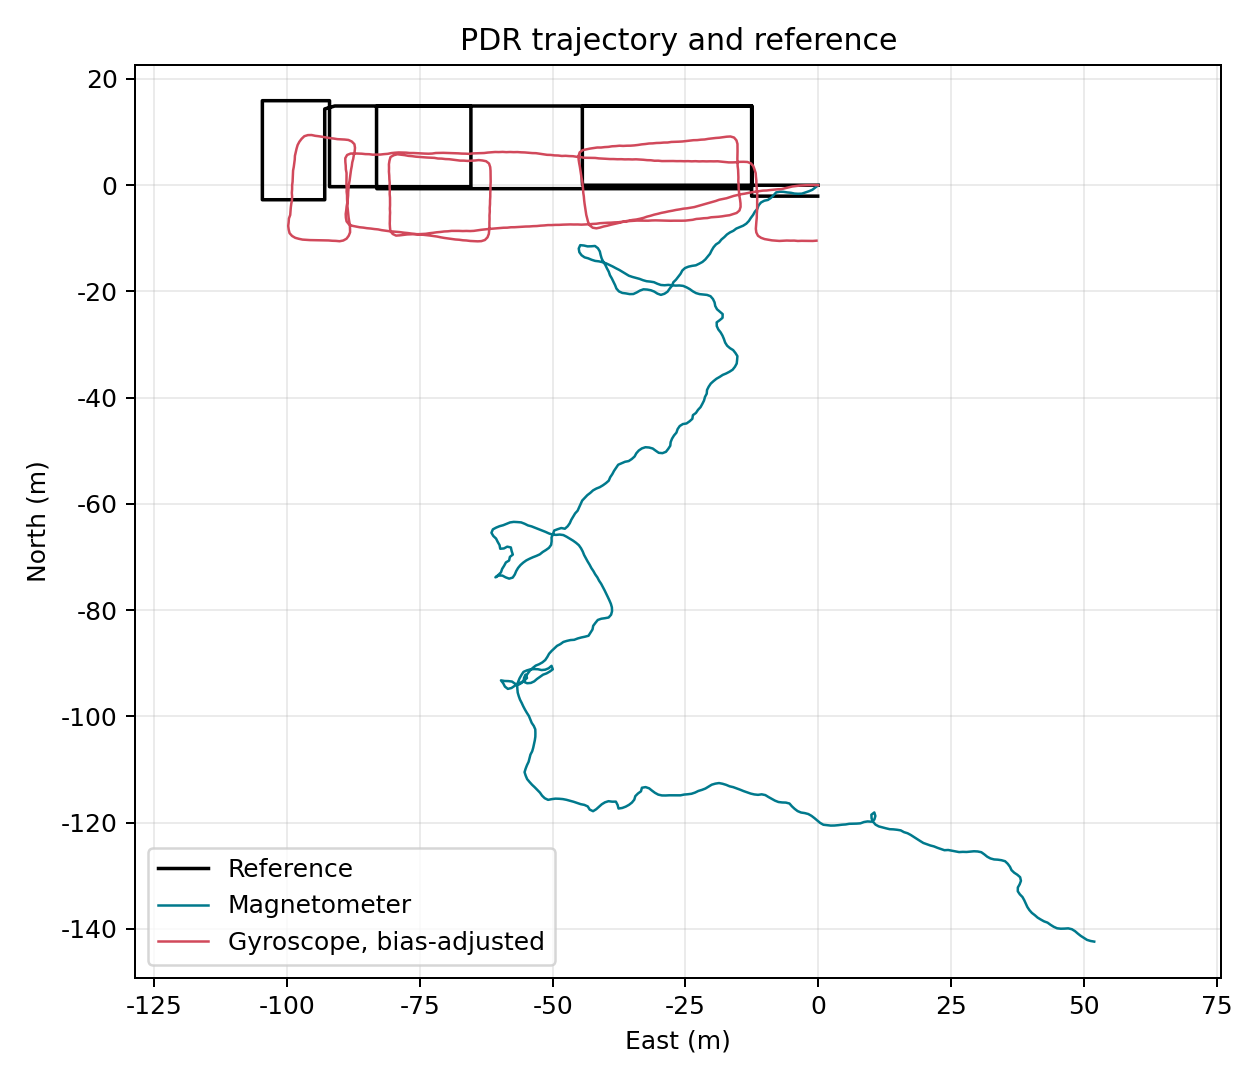
\includegraphics[width=.72\linewidth]{pdr_track.png}
\caption{参考轨迹、磁航向 PDR 与补偿陀螺航向 PDR}
\label{fig:pdr}
\end{figure}
以项目中补偿陀螺轨迹在步伐时刻对参考位置进行比较，误差均值 8.103 m、RMSE 8.381 m、95 分位 10.533 m，末步误差 8.383 m。该误差远大于单步长度，表明仅增加固定的 $0.25^\circ/\mathrm{s}$ 角速度补偿并不足以保证长期轨迹与参考轨迹一致。由于报告使用的是已有 PDR 轨迹输出且没有对起始航向作拟合配准，不能把数值归因于某一项传感器误差；需进一步核查传感器坐标系定义、航向正方向、磁偏角、参考轨迹与采样时钟同步，并对步长和陀螺零偏进行标定。固定步长误差会随步数累积，航向误差则会造成横向漂移。
图~\ref{fig:pdr-raw} 按时间展示程序输出中的三轴加速度、角速度和磁场观测，纵轴分别标出 SI 加速度、弧度每秒角速度及微特斯拉磁场。图~\ref{fig:pdr-signals} 将加速度模及步伐标记、平滑横滚/俯仰和磁/补偿陀螺航向按时间排列。加速度模用于观察步伐检测触发与动态变化；姿态角反映调平后的机体倾斜；航向曲线显示磁方位与陀螺积分在长时间内的差异。所有序列来自项目已保存的 C++ 结果文件，并非原始手机传感器文件重新计算。图~\ref{fig:pdr-error} 给出 592 个检测步时刻的水平误差，横轴为时间、纵轴为与插值参考轨迹的平面距离。误差 RMSE 为 8.381 m，时间变化表明偏差持续存在，因而不能用末点偏差单独描述整段轨迹。
\begin{figure}[htbp]
\centering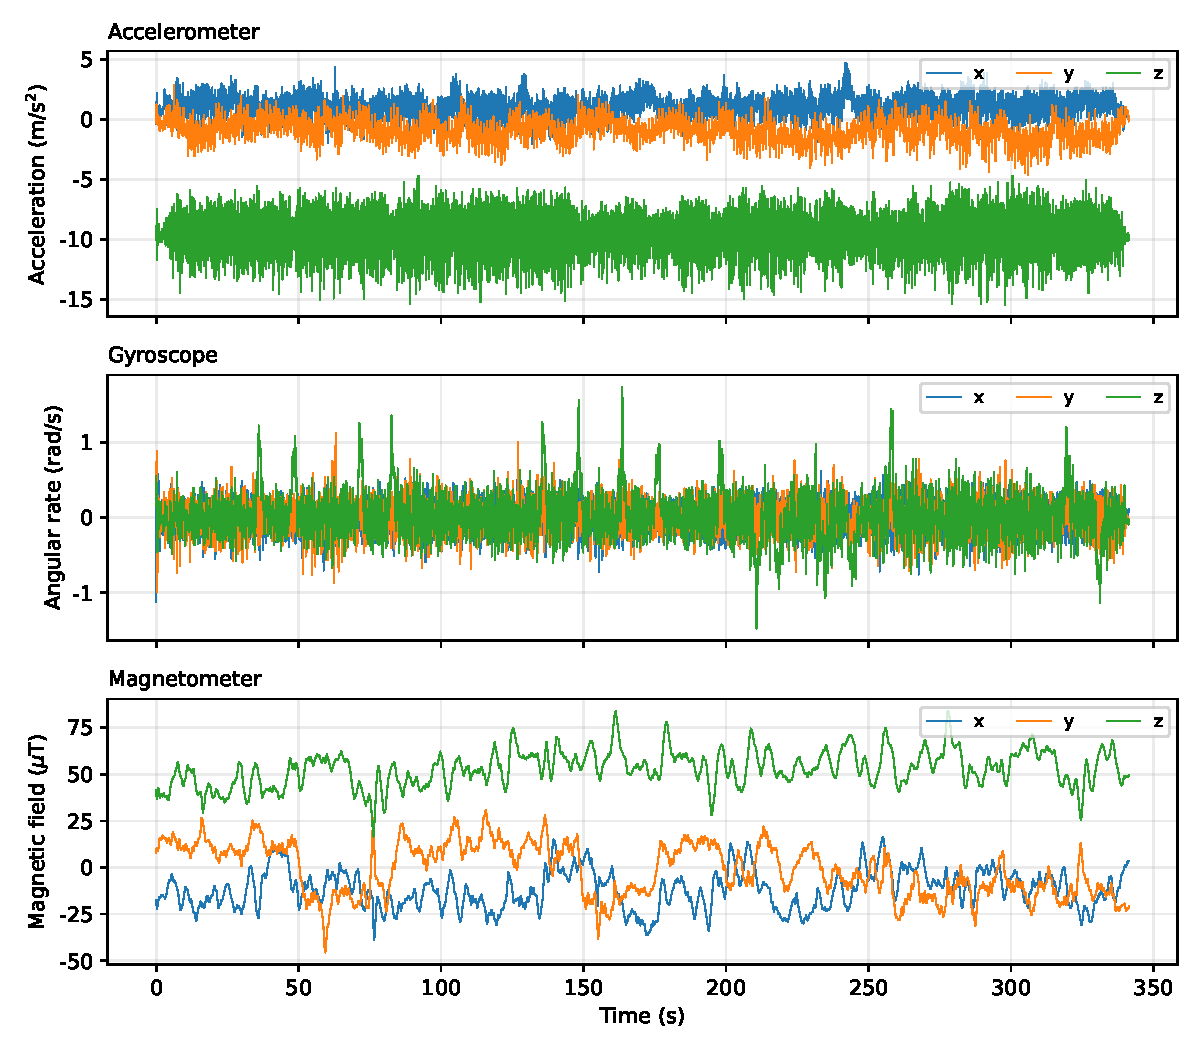
\includegraphics[width=.88\linewidth]{pdr_raw_sensors.pdf}
\caption{PDR 程序记录中的三轴加速度、角速度与磁场观测}
\label{fig:pdr-raw}
\end{figure}
\begin{figure}[htbp]
\centering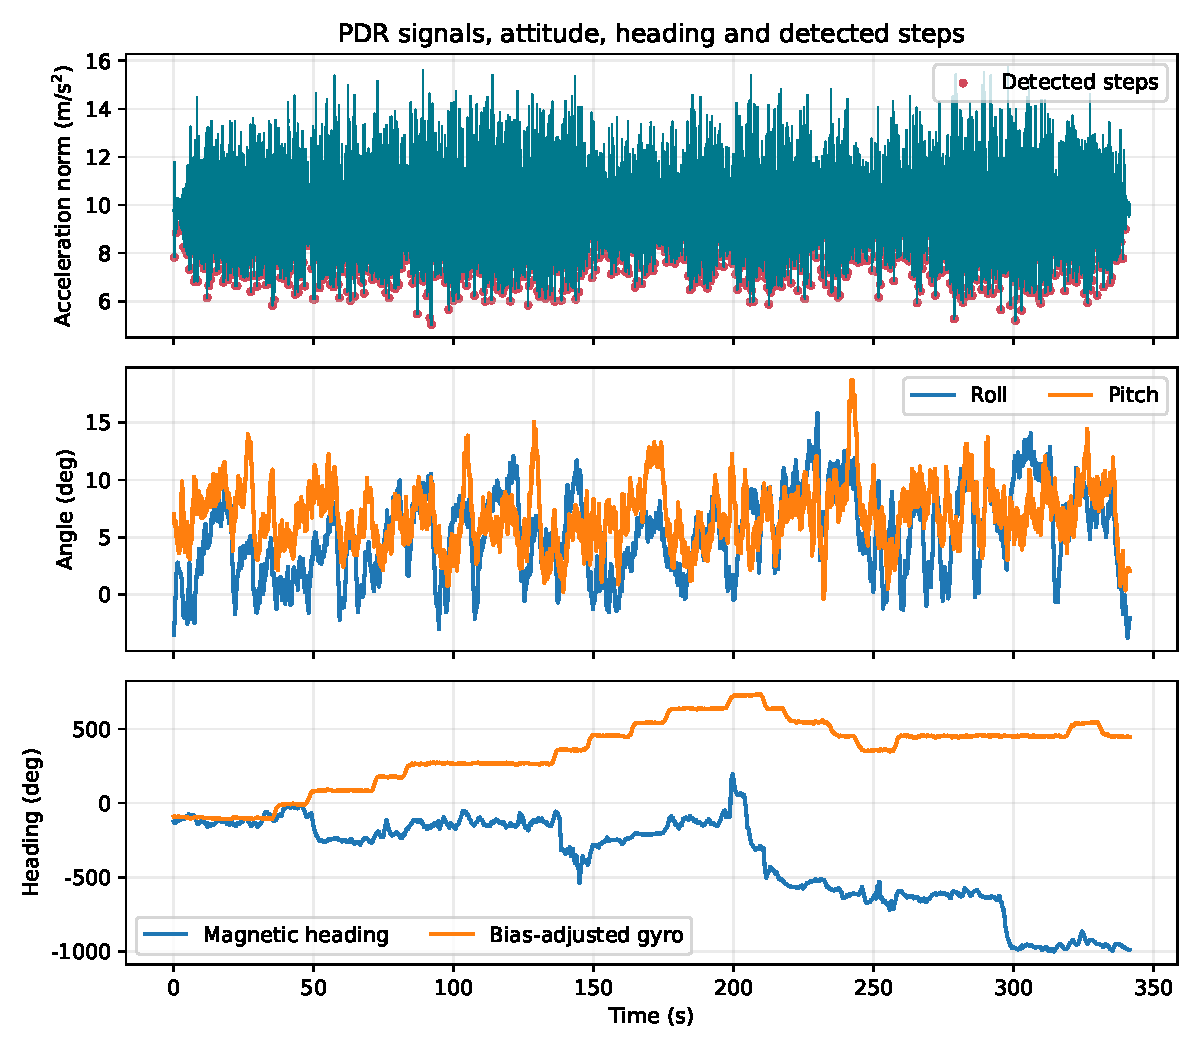
\includegraphics[width=.90\linewidth]{pdr_signals.pdf}
\caption{PDR 加速度模、姿态角、航向与步伐检测时序}
\label{fig:pdr-signals}
\end{figure}
\begin{figure}[htbp]
\centering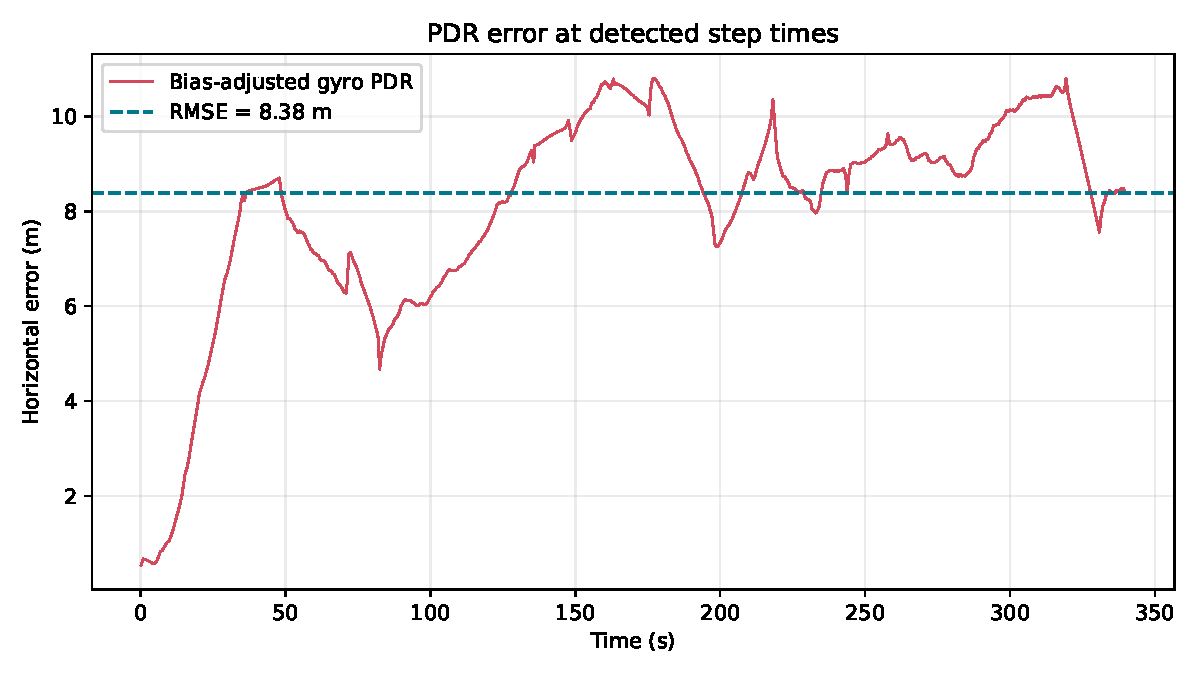
\includegraphics[width=.84\linewidth]{pdr_error_time.pdf}
\caption{PDR 在步伐时刻的水平位置误差}
\label{fig:pdr-error}
\end{figure}

\subsection{UWB 标签二维轨迹与垂向偏差}
实例报告还展示了 UWB 位置轨迹。本项目 tag 2 目录同时提供 C++ 解算结果和真值，可以按时间戳严格匹配而不依赖行序。本次 6,207 条估计中有 5,971 条与 5,971 条真值时间戳相同；仅在该交集上统计水平误差。图~\ref{fig:uwb} 左侧横纵轴为真值/估计的 $x,y$ 坐标（m），右侧横轴为匹配段起点后的秒数，纵轴为水平误差。水平 RMSE 为 0.108 m，均值为 0.084 m，95 分位为 0.189 m。图~\ref{fig:uwb-z} 的上图比较真值高度与估计高度，下图表示逐历元高度误差及其平均偏差。高度平均偏差为 $-0.821$ m，垂向 RMSE 为 0.845 m，说明此组结果适合评价平面轨迹，但三维误差受明显高度系统差影响。当前未找到可核验的 DOP 时序输出，故不仿造实例报告中的 DOP 曲线；UWB 结果文件也属于项目已存 C++ 输出的后处理，不宣称本轮重新运行了 UWB 主程序。
\begin{figure}[htbp]
\centering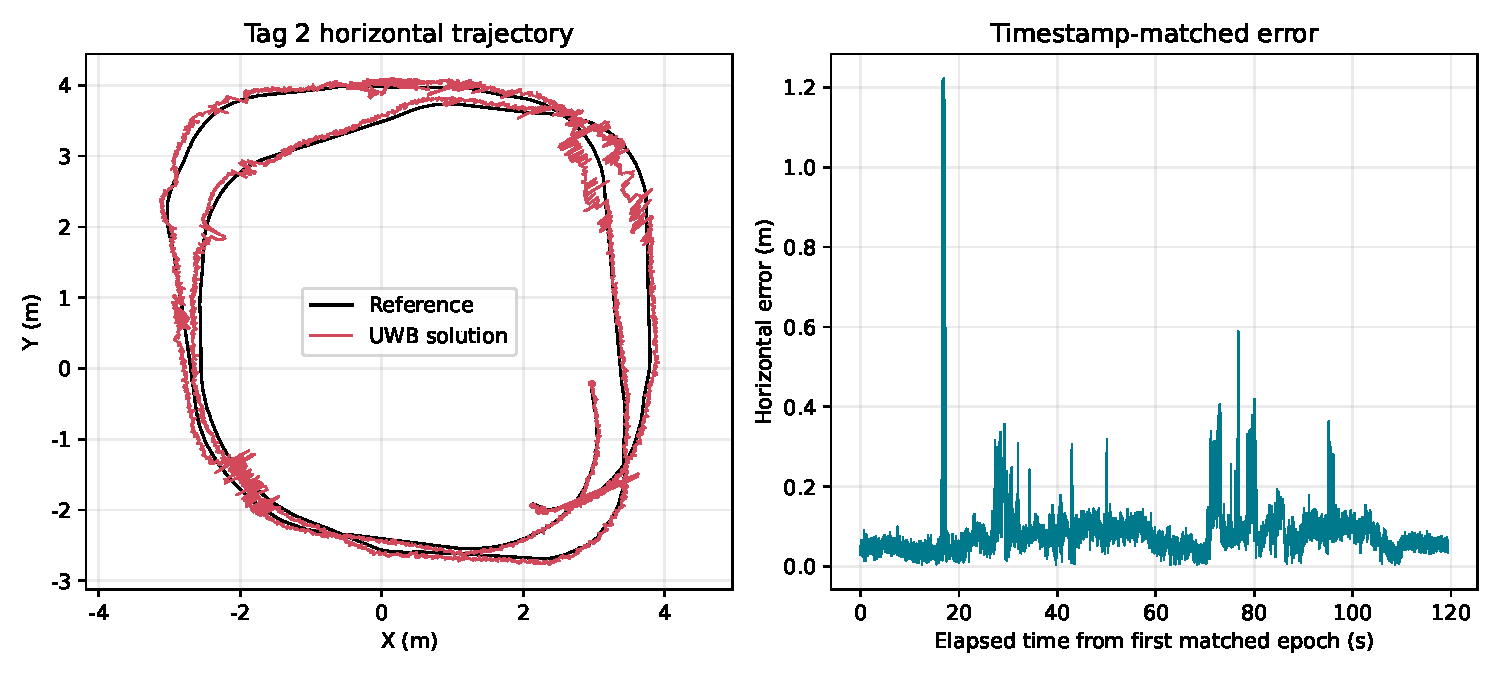
\includegraphics[width=.96\linewidth]{uwb_tag2_track_error.pdf}
\caption{UWB tag 2 平面轨迹及时间戳匹配的水平误差}
\label{fig:uwb}
\end{figure}
\begin{figure}[htbp]
\centering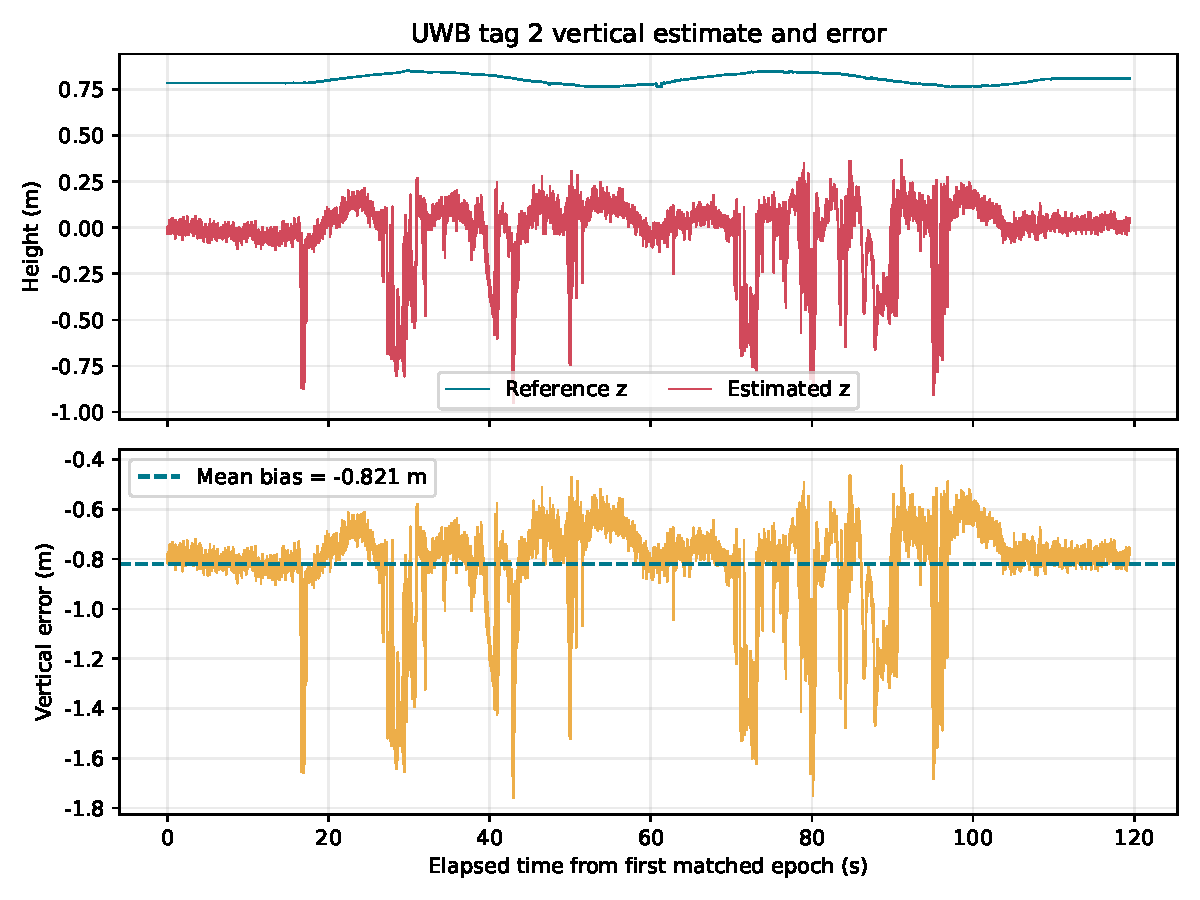
\includegraphics[width=.84\linewidth]{uwb_tag2_vertical_error.pdf}
\caption{UWB tag 2 真值/估计高度及垂向误差}
\label{fig:uwb-z}
\end{figure}

\section{方法比较与讨论}
\begin{table}[htbp]
\centering\caption{三种方法的观测、误差特征与本次证据等级}\label{tab:compare}
\begin{tabular}{p{2.5cm}p{3.2cm}p{4.0cm}p{3.1cm}}
\toprule 方法 & 主要观测 & 主要误差/优势 & 本次结果证据 \\
\midrule 几何距离交会 & 到已知基站的距离 & 几何条件直接影响解算精度；可解释、定位精度高，但要求基础设施和可靠测距 & 对已有教室 C++ 输出重算真值误差 \\
RSS 指纹 & 多 AP 的接收功率向量 & 部署简单、无需测距模型；依赖场景稳定、建库密度与设备一致性 & 从原始训练/测试数据重新计算 \\
PDR & 加速度、角速度、磁场 & 自主连续但位置漂移积累；步长、步检和航向均需标定 & 对项目已有 C++ 结果作真值对齐复核 \\
\bottomrule
\end{tabular}
\end{table}
三种方法的误差指标来自不同场地、不同参考条件，不宜将表~\ref{tab:finger} 与教室误差简单解释为算法优劣排序。距离交会报告的是独立真实参考轨迹下的二维误差；指纹报告的是另一个场地中 50 个离散历元的水平误差；PDR 对齐受到参考轨迹与设备坐标方向的影响。它们说明各方法各自的数据条件下的行为，而非严格控制变量对比。

Android 采集软件说明了手机端数据采集、点号关联和按会话保存的流程，配套 MATLAB 脚本负责传感器、Wi-Fi 与 GPS 数据转换。课程项目 Python 脚本还可对指定会话绘制传感器时序和 Wi-Fi 热点分布。但 Android 示例采集会话与指纹/PDR实验文件不是同一数据集，因此不能把该采集样例的统计混入定位结论。
为展示采集记录实际可用性，图~\ref{fig:android-sensors} 统计会话时间范围内的陀螺仪和加速度三轴样本；文件中分别有 6,841 和 6,782 条记录。图~\ref{fig:android-wifi} 按相对时间汇总 Wi-Fi 扫描记录数，328 次扫描共包含 379 个不同 BSSID，平均每次扫描约 88.4 条 AP 记录；图~\ref{fig:android-rss} 展示按出现扫描次数排序的四个 BSSID 的 RSS 时序，横轴是会话相对秒数，纵轴为接收功率 dBm。不同热点随时间呈现不同幅度的波动，反映接入点可见性和无线信道变化；因文件没有可确认的参考坐标，不将这些 RSS 曲线解释为距离模型或定位误差。数据用于说明传感器与无线观测的采样特征，不与其他采集会话的定位结果混合。
\begin{figure}[htbp]
\centering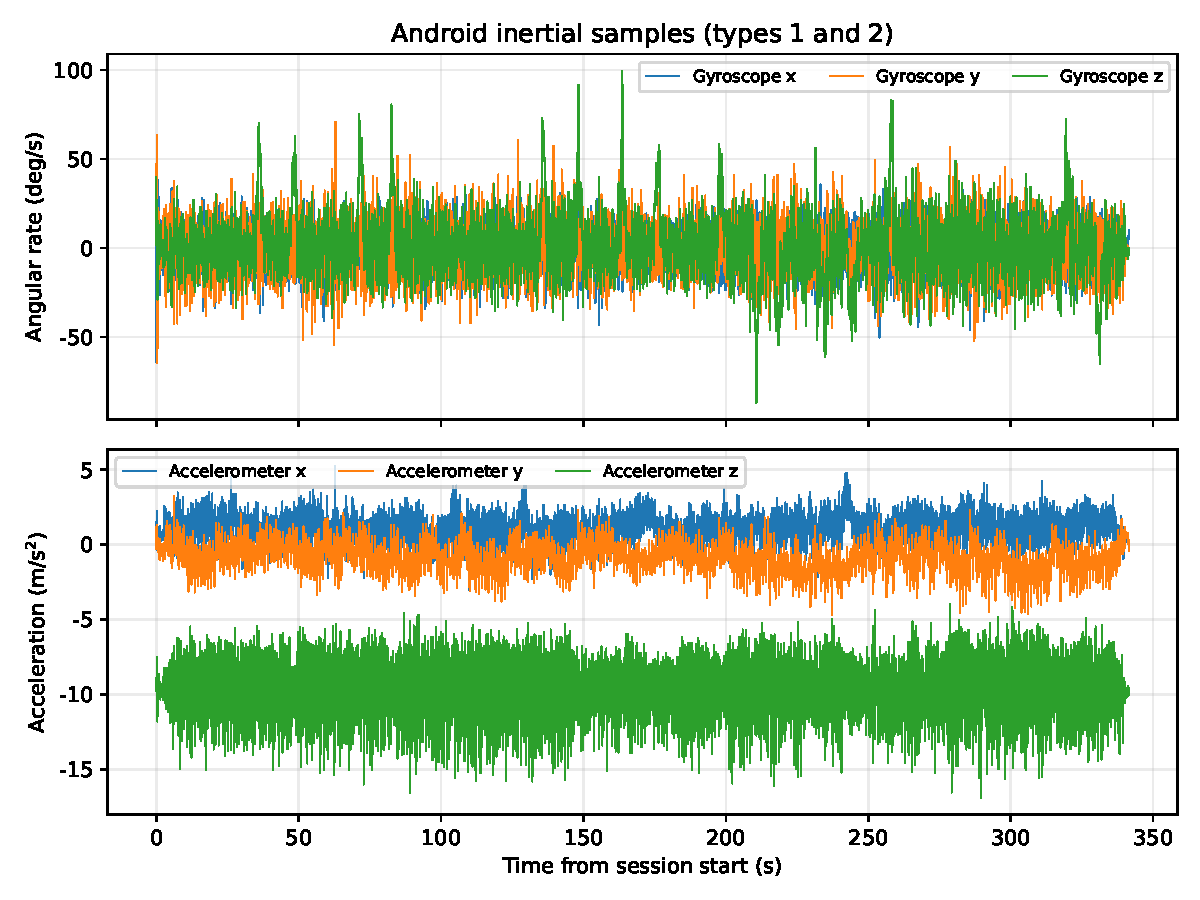
\includegraphics[width=.88\linewidth]{android_inertial_timeseries.pdf}
\caption{Android 样例会话中的陀螺仪与加速度计三轴观测}
\label{fig:android-sensors}
\end{figure}
\begin{figure}[htbp]
\centering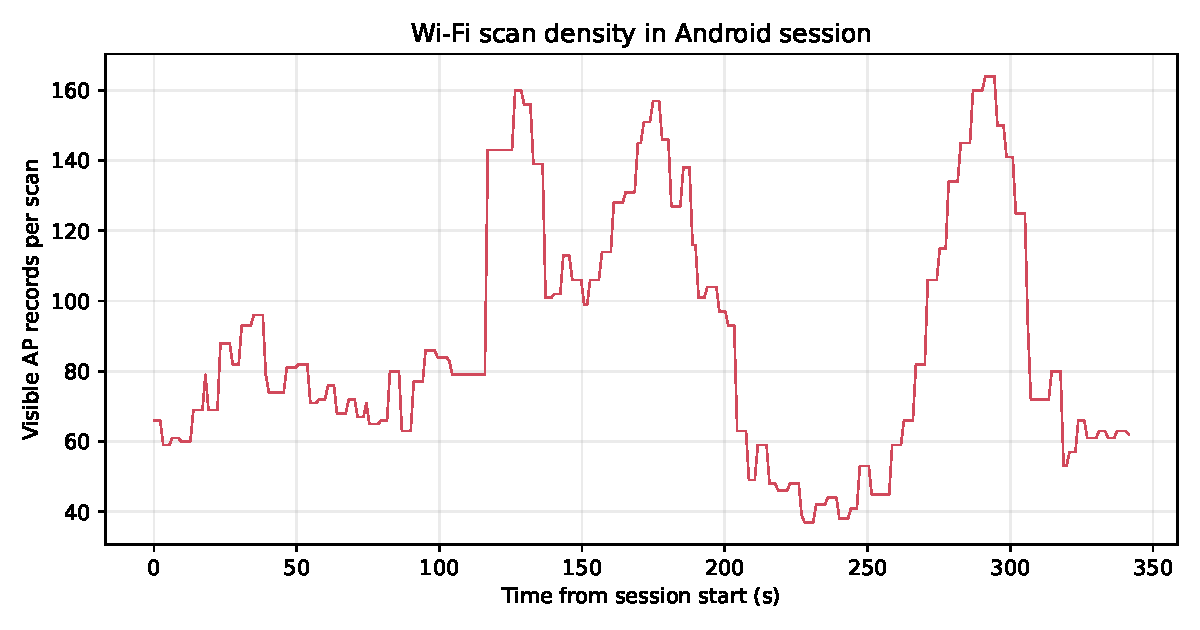
\includegraphics[width=.84\linewidth]{android_wifi_scan_density.pdf}
\caption{Android 样例会话的 Wi-Fi 扫描记录数时序}
\label{fig:android-wifi}
\end{figure}
\begin{figure}[htbp]
\centering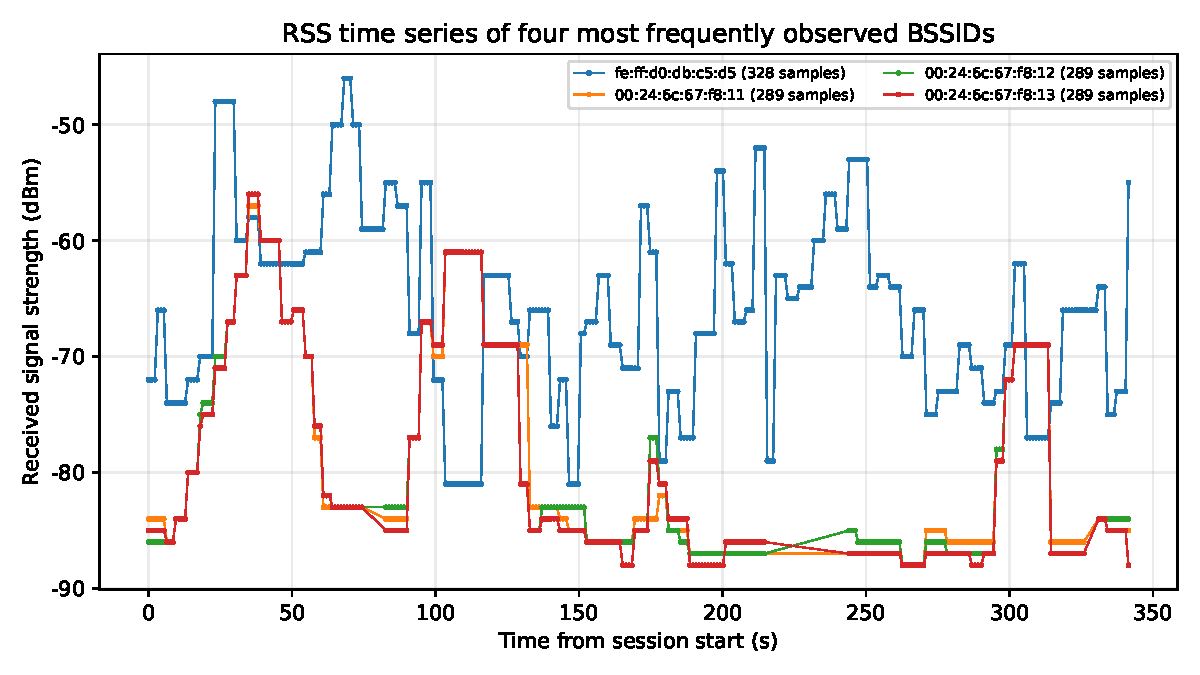
\includegraphics[width=.84\linewidth]{android_wifi_rss_timeseries.pdf}
\caption{Android 样例中出现频次最高的四个 BSSID 的 RSS 时序}
\label{fig:android-rss}
\end{figure}

    \section{实现局限与改进方向}
距离交会的法方程迭代没有按测距精度加权，也没有剔除 NLOS 离群值；改进时应采用基于测距方差的加权最小二乘、鲁棒损失、几何精度因子与残差诊断，并通过独立标定确认基站坐标和设备时间同步。RSS 定位可增加 AP 方差建模、缺失机制处理、设备 RSS 偏差校准以及按轨迹段划分的留出验证；按时间随机拆分会产生空间/时间泄漏风险，应优先采用独立采集段验证。PDR 可标定步长与陀螺零偏，改用自适应步长和磁干扰检测，并在有可信锚点时融合几何或指纹观测来约束漂移。

本次工作范围还有明确边界：除指纹算法外，没有重新执行所有原有 C++ 变体；无人机、UWB、学生无遮挡/遮挡实验未形成新的独立复算结果。原始输出文件的来源版本也未由本轮 Git 历史逐项确认。因此报告将教室/PDR结果称为既有程序输出的复核，不作“本轮完整重跑”的表述。

\section{结论}
本项目形成了从测距、RSS 匹配到惯性航迹推算的互补实验链。指纹算法在给定测试集上实现了 100\% 输出率，水平误差 RMSE 为 1.422 m；教室超声既有解算经参考轨迹复核得到 0.239 m RMSE，测距拟合残差中位数约 9.9 mm；PDR 既有轨迹按步伐时刻与经纬度参考路径对照得到 8.381 m RMSE。测距拟合残差与坐标误差含义不同，而跨实验数据条件也限制了算法横向排名。最值得进一步完成的工作是隔离重跑全部 C++ 程序、统一坐标系/时间基准，并基于独立重复采集开展参数标定和跨场景验证。

\section*{参考资料}
\addcontentsline{toc}{section}{参考资料}
\begin{enumerate}[label={[\arabic*]},leftmargin=2.2em]
\item 室内定位课程课件：\textit{室内定位技术——几何定位}、\textit{室内定位技术——航迹推算}、\textit{室内定位技术——数据库匹配}、\textit{室内定位传感器}，课程提供文件，2026。
\item IndoorPos 项目源码：\url{src/DistanceIntersection/}、\url{src/Fingerprint/}、\url{src/PDR/}、\url{src/Sensors/}，课程实验材料。
\item IndoorPos 实验数据说明：距离交会数据目录下 \texttt{数据格式.md/readme.md}、指纹定位数据及 PDR 数据文件，课程实验材料。
\item Android Sensors 数据采集说明：配套使用文档及 \texttt{DataConvert} MATLAB 转换程序，项目配套材料。
\end{enumerate}


    \clearpage
    \appendix
\section{复算文件与运行说明}
运行 \texttt{python analysis.py} 会重新计算指纹定位及 K 敏感性，并对项目已有 PDR、教室超声和 UWB 输出作时间对齐后处理；Android 采集样例绘制传感器和 Wi-Fi 扫描图。脚本在 \texttt{results/} 输出 CSV，在 \texttt{figures/} 同时输出 PDF 矢量图和 PNG 预览。脚本不会调用原项目主程序，亦不会改写原始输入或既有结果。LaTeX 编译命令为 \texttt{xelatex main.tex}，建议连续编译两次以更新目录和交叉引用。

\end{document}
